\documentclass[b5paper]{article}
%\usepackage[utf8]{inputenc}

%\usepackage{fontspec}
%\setmainfont{Linux Libertine O}

\usepackage{polyglossia}
\usepackage{amsmath}
\usepackage{multirow}
\usepackage{amsfonts}
\usepackage{amssymb}
\usepackage{breqn}
\usepackage[parfill]{parskip}
\usepackage{tikz}
\usepackage{float}
\usepackage{epstopdf}
\usepackage{color}
\usepackage{fontspec}
\usepackage{xunicode}
\usepackage{xltxtra}
\usepackage{fancyhdr}
\usepackage{expex}
\usepackage{bm}

\usepackage{url}

\usepackage{subcaption}

\usepackage[left=1.65cm,right=1.65cm,top=2cm,bottom=2cm]{geometry}
%\chead{\textsc{\small }}
%\rhead{}
%\lfoot{}
%\cfoot{\thepage}
%\rfoot{}
%\pagestyle{fancy}

\makeatletter
\def\blfootnote{\gdef\@thefnmark{}\@footnotetext}
\makeatother

\setmainfont[Mapping=tex-text]{Linux Libertine O}

\newcommand{\todo}[2]{{\textcolor{red}{\bf [#1] #2 }}}
\newcommand{\note}[1]{{\textcolor{blue}{#1}}}

\newcommand{\ns}{Northern Sámi}

\newcommand{\ds}[1]{\textsc{#1}}

\title{Automatic Speech Recognition for \ns\ with comparison to other Uralic Languages} 
\author{Peter Smit \\ \texttt{peter.smit@aalto.fi} \and Juho Leinonen \\ \texttt{juho.leinonen@aalto.fi} \and Mikko Kurimo\\ \texttt{mikko.kurimo@aalto.fi}  \\
[0.5cm]Department of Signal Processing and Acoustics, Aalto University\\}


\begin{document}

\maketitle

\begin{abstract} 
Speech technology applications for major languages are becoming widely available, but for many other languages there is no commercial interest in developing speech technology. As the lack of technology and applications will threaten the existence of these languages it is important to study how to create speech recognizers with minimal effort and low resources.

As a test case, we have developed a Large Vocabulary Continuous Speech Recognizer for \ns, an Uralic language that has little resources for speech technology available. Using only a limited audio data, 2.5 hours, and the \ns\ Wikipedia as language model we achieved 7.6\% Letter Error Rate (LER). With a language model based on a higher quality language corpus we achieved 4.2\% LER. To put this in perspective we also trained systems in other, better-resourced, Uralic languages (Finnish and Estonian) with the same amount of data and compared those to state-of-the art systems in those languages. 
\end{abstract}

\section{Introduction}

The field of speech recognition is maturing, as companies start to actively use and sell products that utilize Large Vocubulary Speech Recognition (LVSCR). Especially the creators of operating systems for mobile devices incorporate methods into their products to operated devices using voice.

These commercial applications however, are only focusing on small fraction of the available languages. Other languages do not have the available resources, in the form of data and expertise, and it is often not commercially viable to create this resources. Especially minority languages and languages from developing countries receive only minor academic and commercial interest for the development of LVCSR systems. \cite{besacier2014automatic}

One for these under-resourced languages is \ns, the largest of the nine Sámi languages with approximately 25 000 speakers. It belongs to the Uralic language family. \cite{ethno18}

Like other languages in the Uralic language familiy, like Finnish and Estonian, it is highly morphological as the language uses independent suffixes extensively. This poses challenges for speech technology applications as the number of inflections, derivations and compoundings cause the size of the vocabulary to be enourmous, especially compared to the languages in the Indo-European family \cite{karlsson1982}.  The great different number of words causes especially problems in the estimation of language models, which can not produce any words beyond those seen in the the training data. 

\ns\ is an under-resourced language as there are little corpora of spoken and written language available, and financial resources to collect these data are limited. Even though there is active linguistic research on \ns, there are limitations to the expert resources avaible for speech recognition, such as pronunciation dictionaries. 

To combat the challenges of building an LVCSR system for an under-resourced language we have employed different techniques. First we used `found data' for building the acoustic and language models. For the acoustic model we needed to bootstrapped from a bigger related language (Finnish). For the language model we used subword units (morphs) to increase the coverage of the language. Similar techiques have been used in \cite{besacier2014automatic,viet2009}.

To project a possible upper-bound on the recognition accuracies possible for \ns, we also have produced systems for Finnish and Estonian, using the same quantities of data for comparison. Comparing these to the state-of-the art systems for Finnish and Estonian will give a good estimate of the possible gains before more \ns\ data is gathered.

This work is an extension of \cite{leinonen2015}.

\subsection{WikiTalk and DigiSami}
Another motivation to build a recognizer for \ns\ is to utilize it as part of  a spoken dialogue system in the WikiTalk application \cite{wilcock2013wikitalk}. This is one part of the DigiSami project which ``is a research project at University of Helsinki which aims to support content generation of less resourced languages with the help of language technology''. Currently, the biggest dangers to Sami language are the disappearance of the traditional lifestyle and work of Sami culture, and emigration of Sami people from their old living areas. However, there are also studies and discussion on using new technologies to revitalize languages \cite{eisenlohr2004language}. In \cite{jokinen2014open}, the author describes revitalization for the \ns\ language using the WikiTalk application. In WikiTalk, the idea is to have users (children or adults) find out more about subjects that interest them by discussing with the humanoid robot Nao. They can ask for more information on the subject and then Nao will read them the related Wikipedia article \cite{jokinen2014multimodal}. The recognizer is a first part to building this end-to-end system.


\section{ASR for under-resourced languages}
The majority of the state-of-the art methods in Large Vocabulary Speech Recognition require large amounts of data and expertise. 

Firstly, a great number of high quality spoken utterances have to be collected and correctly transcribed. In the case of Speaker-Independent (SI) systems, a system that can recognize anyone who speaks the target language, utterance from many different persons are needed. For Speaker-Dependent (SD) systems, a system that can only recognize the voice of the person that spoke the training data, only a few hours of voice and transcriptions are required.

The second required dataset is a large corpus of written text, preferably in the same style and domain as what should be recognized by the system. This corpus should at least contain all common words in their expected contexts in order to train a good language model.

Lastly, a normal speech recognizer needs a pronunciation dictionary. A list of all possible words with all their possible phonetic transcriptions. Also needed is a list of questions that separate the phonemes in different groups, this is used in acoustic model training to share probability distribution with decision tree clustering.

As none of the above data and expertise are readily avaibable for an underresourced language, alternatives have to be developed. In the case of transcribed audio data, a good resource would be audio books. Projects such as Librivox have freely available audiobooks in many languages, although the quality varies. Using a temporary acoustic model and basic text processing techniques these audiobooks can be automatically segmented into sentence-long utterances that are suitable for training a minimal speaker-dependent model.

Also language data is often freely available online, though not necessary high-quality or in usable form. Web-scraping \cite{scannell2007crubadan} can give a rudimentary dataset for training a language model. Also sites like wikipedia have often big collections of easily available text. The main problem with this `found' datasets is that the style and topic of the language data found does not match with the actual sentences spoken. Also, the datasets might contain foreign language segments, symbols or abbreviations that dillute the usability.

The pronuciation dictionary requires normally a great effort and linguistic expertise. One solution is to model the graphemes (letters) of the words directly, instead of using the actual phone they represent in the words \cite{kanthak2003multilingual}. In languages such as English this would not give very good results as graphemes can have very different realizations. Consider for example the words `Tough' and `Though', in writing very similar words, but when spoken very different. In the Uralic languages studied here though, a grapheme-to-sound system would work very reasonable as in general every grapheme is only realized as a single distinct sound.

Lastly, the phoneme question set is a small dataset that can only be made by a language expert. Altough there are algorithms avaible that can replace this set altogther \cite{darjaa2011effective}, this is often undesirable as it effects the systems effectiveness. Another method is to take the phoneme set of a very closely related language, and alter it slightly to reflect the correct set for the target language. This can be often done with only minimal expert effort.

Eventhough there is a (partial) solution to all the expensive data needs, all these solutions do limit the resulting speech recognizer in different ways. In the case of state-of-the art ASR systems, always more, higher quality, in domain speech and language data and expertise would improve the system signficantly (up to a certain point). There are however usable systems to be made in the under-resourced situation, with the most limiting factor being that SI systems are unattainable as the number of speakers is too low.




%	\section{UNUSED TEXT}
%	
%	This paper introduces a new speech recognizer for \ns, the largest of the nine Sami languages with about 20 000 speakers. \todo{Juho}{Cite}  Sami is a morphologically rich language in the Uralic group, and consequently it suffers from the same issues as Finnish speech recognition: inflection and compounding add a huge number of words to the lexicon. \ns is also an under-resourced language, so it is not feasible to collect enough data for a corpus that contains natural occurrences of all the different word forms. Another issue is the lack of expert help, for instance there is not enough resources to build a proper pronunciation dictionary for Sami, and therefore here, and in other model training phases, this paper introduces useful generalizations and unsupervised learning as techniques that could be applied to other under-resourced languages as well.
%	
%	Words are the most common unit for n-gram language models, and they work very well for analytic and isolating languages such as English. However, they are not the best choice for synthetic languages such as Finnish, Estonian or Sami. In these type of languages additional information is mostly added to the stem of the word, instead of using prepositions, postpositions or other parts of speech. Therefore, conferring information that might take many English words could be done with just one in Sami, for example TELL AN EXAMPLE. Thus, using segmented word fragments called morphs was tested as a language model unit for the recognizer. Morphs get their name from morpheme, which is the smallest grammatical unit of a language. In this paper both unsupervised and supervised learning for the optimal segmentation was tested, which resulted in morphs that represented grammatical segmentation, and ones that were generated to purely optimize the cost function of the segmentation tool, Morfessor Baseline 2.0 \cite{virpioja2013morfessor}. 
%	
%	Both these new language model units and words are compared to see which produces the best results in terms of error rates, both word error rate (WER) and letter error rate (LER). To make the results somewhat comparable, the total size of the language model will be restricted.
%	
%	\section{Used data}


\section{Acoustic modeling}
\label{sec:align}
The Acoustic Modeling part of the speech recognizer was done with a standard Hidden Markov model with Gaussian mixture models as emission distribution (HMM-GMM). Mel Frequency Cepstral Coefficients were used as input features. 

The audio data is prepared by splitting the audio files (originally chapter length or similar) into sentence utterances. This is done by doing Baum-Welch forced alignment with a temporary speech recognition model. The temporary speech recognition model was created by taking a well trained Finnish model and mapping the Finnish phonemes to the one of the target language. In later iterations the best speech recognition model of the language was used to do the forced alignment again, resulting in a perfect split of training utterances.

The HMM-GMM model is trained using multiple iterations of Baum-Welch, maximum likelihood estimation. To manage the model complexity Gaussians were shared between different states using decision tree clustering. The modeling unit of the model is a tri-state, tri-phone. This means that all phones with a different preceeding and succeeding phone are modeled in their own state, as well as the start, middle and end of every phone.

Although there are different tuning possibilities in the acoustic model, specifically that control the number of parameters (Gaussians) in the model, the defaults were used as small experiments showed no improvements in different values. In Section~\ref{sec:compexp} the number of Gaussians for different models are reported.


\section{Language modeling}

The language model is an important part of any speech recognition system. Even though theoretically a good acoustic model with lexicon could be enough to output words, a model that takes the word context into account to predict the right output is essential. For languages where different words can have the same pronunciation it is also essential in picking the right word given a pronunciation. 

N-gram models predict the output of the next word given the `N - 1' previous words. The main issue however with using words as a language model unit for a synthetic language is that to decrease the out-of-vocabulary (OOV) rate to a manageable percentage, a huge lexicon is needed. Since OOV-rate is the minimum WER possible, a OOV-rate much less than 10\% would be necessary. For an English speech recognizer this can be achieved with already with 20 000 words for OOV-rate of 2.4-2.7\% and with a vocabulary of 40 000 words OOV-rate less than one percent is achieved \cite{woodland19951994}. In contrast, a Finnish recognizer needs a 410 000 word vocabulary to have an OOV-rate of 4.0-7.3\% \cite{hirsimaki2006unlimited}.

The alternative to using an word based model a subword model could be used. A subword model builds word out of a smaller set of word fragments. The word fragments can be particular effective in agglunative languages or languages with a lot of compound words, as not all combinations of word fragments have to be seen in a corpus to be output by the model. If the word fragments are choosen correctly the OOV-rate can be close to zero, even for smaller language data corpora.

\subsection{Morfessor}
Morfessor is a machine learning tool that uses a statistical model to split text into smaller fragments, which can be used for language modelling \cite{creutz2007unsupervised}. This resembles closely the splitting of words into it smallest informational units, morphemes. The basic working is inspired by Minimum description length.

The three components of a Morfessor are the model, cost function, and training and decoding algorithms. The model contains the lexicon: properties of the morphs, the written form of the morph itself and its frequency, and the grammar: how the morphs can be combined into words. Morfessor cost function is derived from a MAP estimation with the goal of finding the optimal parameters $\bm{\theta}$ given the observed training data $\bm{D}_W$:

\begin{equation}
\bm{\theta}_{MAP}=\operatorname*{arg\,max}_{\theta}P(\bm{\theta}|\bm{D}_W)=\operatorname*{arg\,max}_{\theta}P(\bm{\theta})P(\bm{D}_W|\bm{\theta}).
\end{equation}

The cost fuction to minimize becomes the minus logarithm of the product

\begin{equation}
L(\theta, D_W)=-log p(\theta)-log p(D_W|\theta).
\end{equation}

The purpose of this is to generate a small set of morphs that represents the words in the training corpus compactly. If only letters were used as morphs the set of would be small but representing the corpus with individual words would be cumbersome. In contrast using whole words as morphs would result in a large set of morphs so the optimal solution is somewhere in between. However, individual letters are added to the morph set so even previously unseen words can always be segmented.

A greedy search algorithm is used to find the optimal segmentation of morphs for the training data. One word is selected at a time and all different segmentations are tried, with the one that best improves the unsegmented part chosen and applied to all the other words. When the best model is found it is used to segment the LM training corpus with the Viterbi algorithm. This result can be used to generate n-gram models with morphs as LM units.



\subsection{N-gram modeling}
Although basic N-gram modeling with Knesser-Ney smoothing \cite{chen1996empirical} is the most common technique for building word n-gram models. Unfortunately standard tools have problems with (correctly backing off) deep n-gram language models which are needed when subword units are used. Models that are not correctly pruned are often too big for practical use or do not generalize wel because of overtraining.

\cite{siivola2007growing} has created methods to overcome this limitiation of standard n-gram tools and it is the defacto standard for building higher order n-gram models for subword units.

%Also for For decoding we have used the AaltoASR decoder, which is specialized in decoding morph-language models with deep contexts.


\section{Experiment setup}

%\note{we don't have to explain acoustic modeling, language modelling etc. We do need to tell what recognizer we used (AaltoASR) and what features it has (MFCC's, Gaussian-mixture HMM's, type of decoder). Same for language modeling tools}


The system the experiments were carried out on was AaltoASR \cite{hirsimaki2009importance}\cite{pylkkonen2005efficient}. It uses context-dependent triphones with diagonal Gaussian mixture models (GMM) as emission distributions and the speech features itself are extracted with Mel-frequency cepstral coefficients (MFFCs). 

Both words and subword units were used for language modelling. The subword unit models were created with Morfessor 2.0, an implementation of the Morfessor Baseline algorithm\cite{virpioja2013morfessor}. 

Variable length n-grams are used for language modelling generated with both SRILM \cite{stolcke2002srilm} and VariKN \cite{siivola2007growing,siivola2007morfessor}. The decoder was a one-pass using token passing principles and hence time-synchronous. In addition, beam search complemented with a language model look-ahead is applied \cite{ortmanns1997look}.

%
%\subsection{Acoustic modelling}
%
%Aalto university's speech recognizer is like most speech recognizers in the sense that it uses hidden Markov models (HMM) to model triphones which have use as their emission distributions Gaussian mixture models (GMM). In Finnish, which is a phonetic language, the phonemes of the triphones are generated by just assuming that every letter represents a single individual phoneme. Based on this assumption a lexicon is built. This approach is also used for Sami since it too is a phonetic language and there are not enough resources for building a proper pronunciation dictionary. 
%
%\subsection{Language modelling}
%
%Maybe just a little bit of something, most in the actual section.
%
%
%\subsection{Decoding}
%
%The decoder used in AaltoASR is a "one-pass time-synchronous decoder using re-entrant prefic-tree and token passing principle". It is optimized for Finnish but otherwise language independent. Since the main language model units in Finnish speech recognition are morphs, one problem with the decoding becomes the context-dependent phonemes at the morph boundaries, and the need create a specific model for word boundary prediction. Other issue with Finnish are the double letters for which duration modelling needs to be applied. To limit the amount of transitioning modelling between context-dependent phonemes cross-word network is embedded in the search network. \cite{pylkkonen2013towards}\cite{hirsimaki2006unlimited} All of these solutions will also be used for the decoder for Sami, since morphs will also be tried for it, and it as three different vowel lengths and double consonants. A language model lookahead is also implemented to use the LM probabilities as soon as possible to prune unlikely hypothesis before applying the full computationally heavier language model. This study suggests this length, we will use this. since morphs.
%
%\section{Language modelling}
%
%n-gram, lexicon, words, morphs, morfessor. 
%
%N-gram word models are the most popular method for language modelling. They will also be used here, except using morphs instead of words will also be tested. Since in Sami the amount of word types rises very quickly with increasing corpus size (maybe tests about this with the larger corpus?), limiting the vocabulary might become needed, so tests are done to see its effect on the error rates, and n-gram amounts (speed). For segmenting words into morphs both supervised and unsupervised methods are tested.
%


%\section{Dealing with under-resourced ness}



%\subsection{Lexicon /\ pronunciation dictionary}
%
%maybe more carefully if needed. These people might actually want to see the letter-to-IPA-AaltoASR phoneme table?
%





\section{\ns\ ASR evaluation} 
\label{sec:samiexp}
The audio data used for the \ns\ recognizer came from the UIT-SME-TTS corpus\footnote{Provided by the University of Tromsø}. The Male audio data was 4.7 hours and the Female data 3.3 hours. As we needed to separate data for development and evaluation only 75\% was used for training; 3.5 and 2.5 hours respectively.

The initial recognition model was created by using a Finnish model. With this model the audio data was split into sentences and trained with the procedure described in Section~\ref{sec:align} two speaker dependent systems, one for the male and one for the female speaker (resp. SM1 and SF1). These models are Speaker-Dependent models; they are only usable for the speaker that the system is trained for. As there is only data from two speakers available this was the only option. 

For language model we evaluated both word and morph n-gram models. We used as text data the training sentences together with the \ns\ wikipedia dump (\ds{Train+Wiki}).

The results for basic recognition are shown in Table~\ref{tbl:samibasic}. Besides the standard Word Error Rate (WER), also the Letter Error Rate (LER) is reported, which is common for speech recognition experiments on languages with a high morphological complexity such as \ns, Finnish and Estonian.

\begin{table}[!h]
\centering
\begin{tabular}{ll|rrr|rrr}
& & \multicolumn{3}{|c|}{\textbf{Speaker SF1}} & \multicolumn{3}{|c}{\textbf{Speaker SM1}} \\
 \textbf{Unit} & \textbf{Toolkit} & \textbf{5-gram} & \textbf{7-gram} & \textbf{9-gram} & \textbf{5-gram} & \textbf{7-gram} & \textbf{9-gram}\\\hline
 words & SRILM & 52.9 / 12.7 & 52.9 / 12.7& 52.9 / 12.7&48.6 / 11.1 & 48.7 / 11.1 & 48.7 / 11.1\\
morphs & SRILM & 40.0 /  9.0 & 39.9 / 9.3& 39.1 / 9.1 & 37.6 / 8.5 & 36.8 / 8.4 & 37.3 / 8.5 \\
 morphs & VariKN  & 38.4 / 8.6& 38.5 / 8.7  & 37.6 / 8.7 & 35.4 / 8.1 &  33.7 / 7.6 & 34.1 / 7.9 \\
%DST & words & SRILM & & & & & & \\
%DST & morphs & SRILM & & & & & & \\
%DST & morphs & VariKN  & & & & &  & \\ 

\end{tabular}
\caption{ASR recognition results for the Sami SD recognizers. Word Error Rate / Letter Error Rate reported.\label{tbl:samibasic}}
\end{table}


The first observation is that the SM1 recognizer is slightly better than the SF1 recognizer. This is most likely caused by the fact that there was more data available for the training of the acoustic model.

Just like in other uralic languages, the morph based language models are having much lower error rates then the word based models. Looking to the  the OOV-rates in Table~\ref{tbl:samioov}, it confirms that out of vocabulary words are a big problem for using word based lanuage models in \ns.

\begin{table}[!h]
\centering
\begin{tabular}{lrr}
& Word & Morph\\\hline
Female &  22\% & 0 \% \\
Male & 20 \% & 0 \%\\
\end{tabular}
\caption{Out-of-vocubulary percentages for the Female and Male testsets. \label{tbl:samioov}}
\end{table}


For word based models there is no effect on using higher order models. Figure~\ref{fig:samiperf} shows the results for the SM1 system, with the \ds{Big} sami language model, model trained from appr 12 million word tokens of data from `Den samiske textbanken'. For the word models there is no change in performance after the 3rd order ngrams. For VariKN morph-based models there are clear effects on using higher order models. This is because in order to model the same context as a word model, more units of a subword model are needed. SRILM does not do very well on this morph data, which is caused by the limitited pruning/growing algorithms of SRILM.

The best Word Error Rate on the \ds{Big} language model for the SM1 system is 18.2\%, the best Letter Error Rate 4.2\%. 

\begin{figure}[!h]
\centering
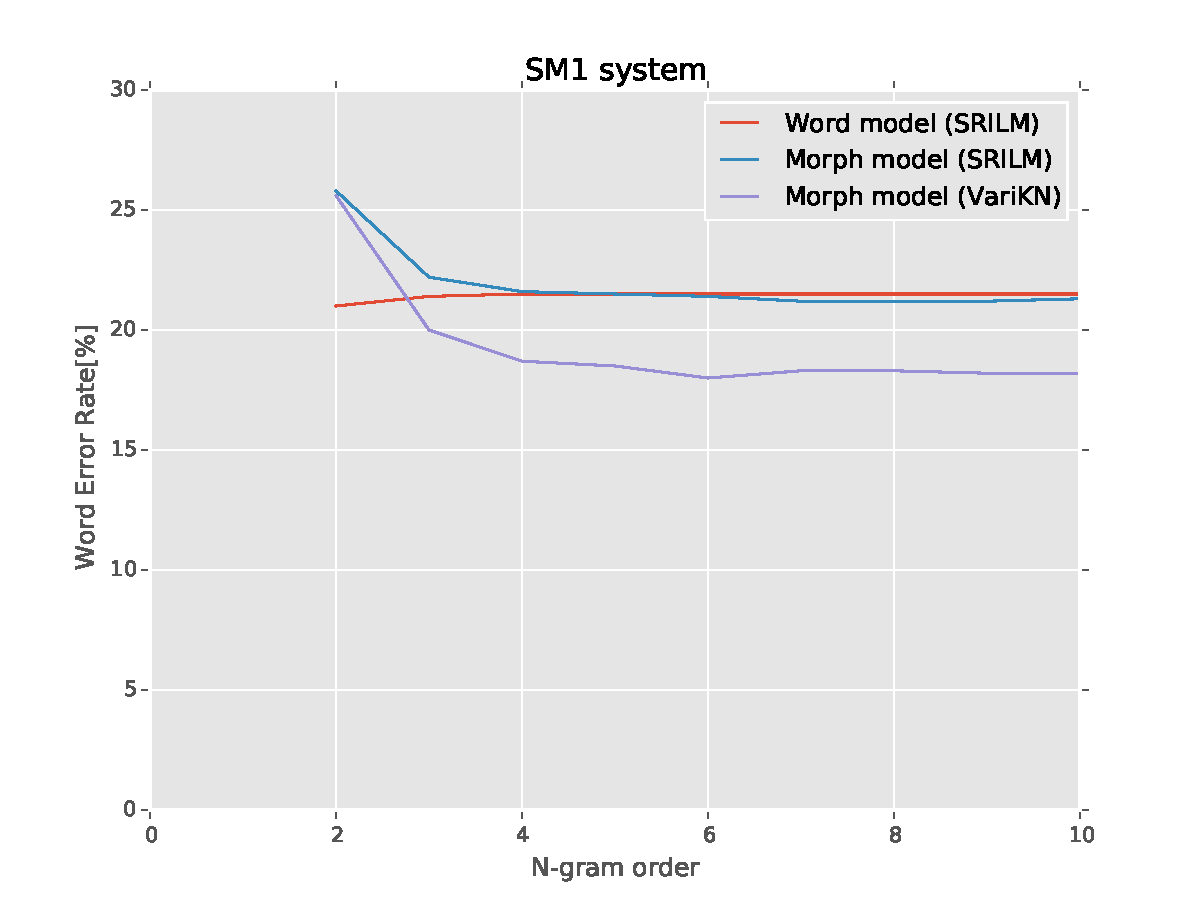
\includegraphics[width=\textwidth]{figures/sme1}
\caption{Word error rates for the SM1 system with the \ds{Big} language model.}\label{fig:samiperf}

\end{figure}



%The last observation is that the VariKN toolkit does a better job in creating a high-order ngram model for morph models. This is expected as it is specifically designed to be used for this purpose.




%\begin{figure}[!h]
%\centering
%\begin{subfigure}[b]{.4\textwidth}
%
%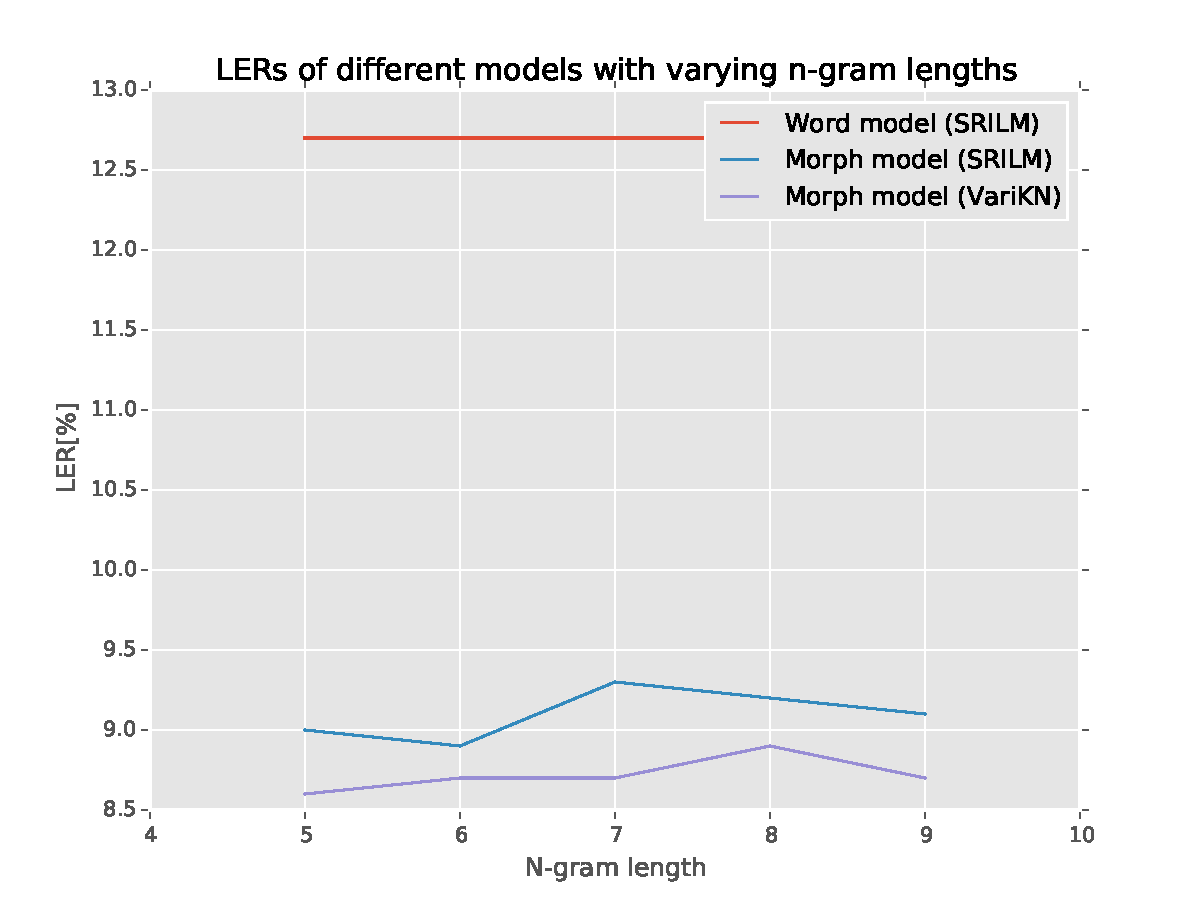
\includegraphics[width=\textwidth]{figures/smeF-complete_wikipedia-ler}
%\caption{Female data - letter error rate}
%\end{subfigure}~
%\begin{subfigure}[b]{.4\textwidth}
%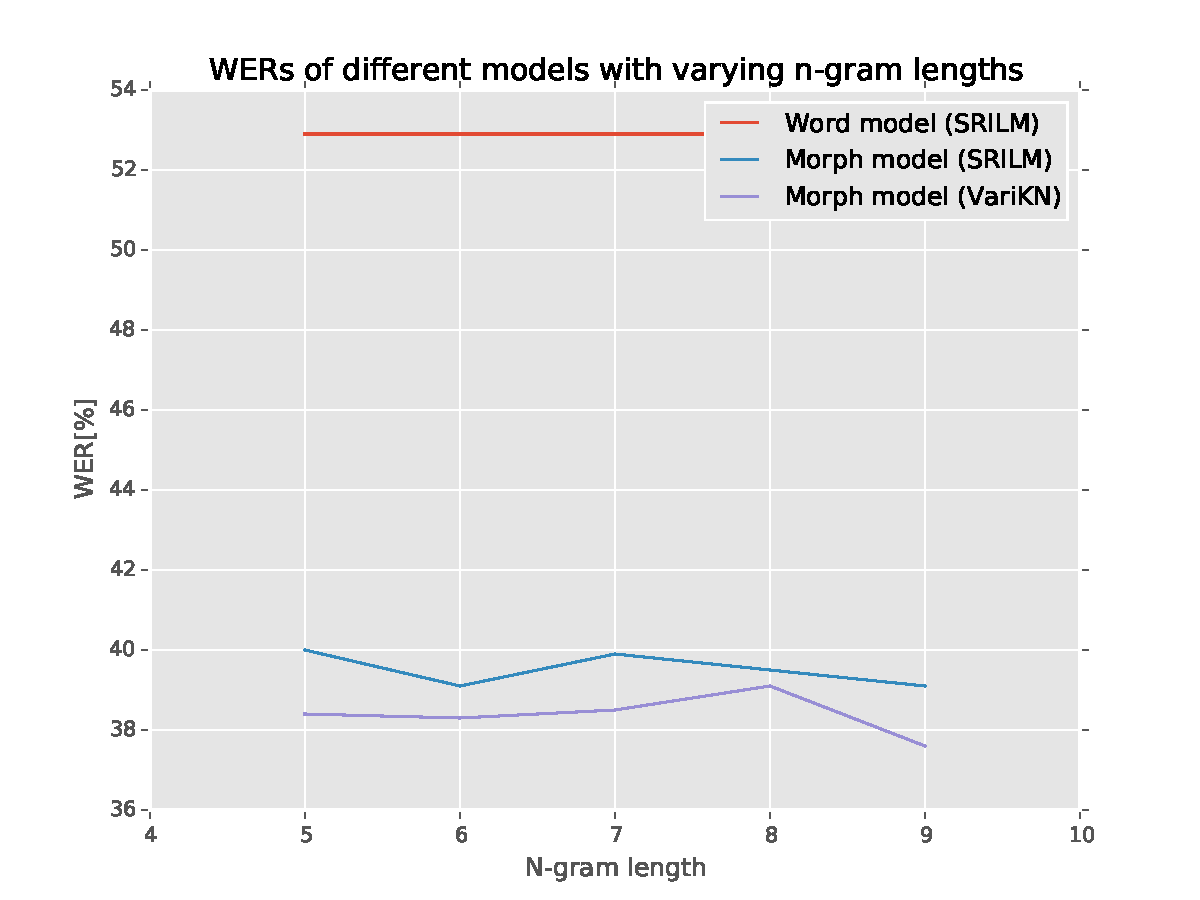
\includegraphics[width=\textwidth]{figures/smeF-complete_wikipedia-wer}
%\caption{Female data - word error rate}
%\end{subfigure}
%
%\begin{subfigure}[b]{.4\textwidth}
%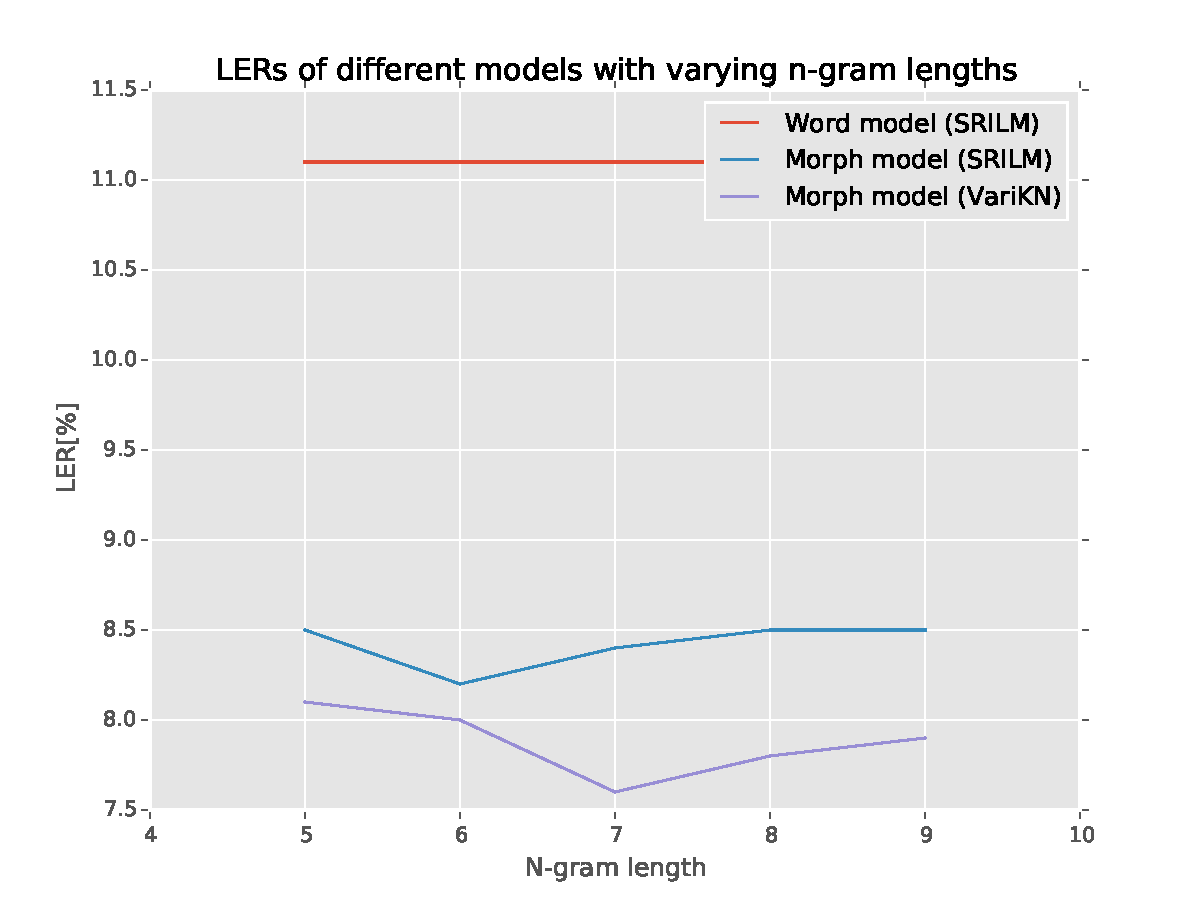
\includegraphics[width=\textwidth]{figures/smeM-complete_wikipedia-ler}
%\caption{Male data - letter error rate}
%\end{subfigure}~
%\begin{subfigure}[b]{.4\textwidth}
%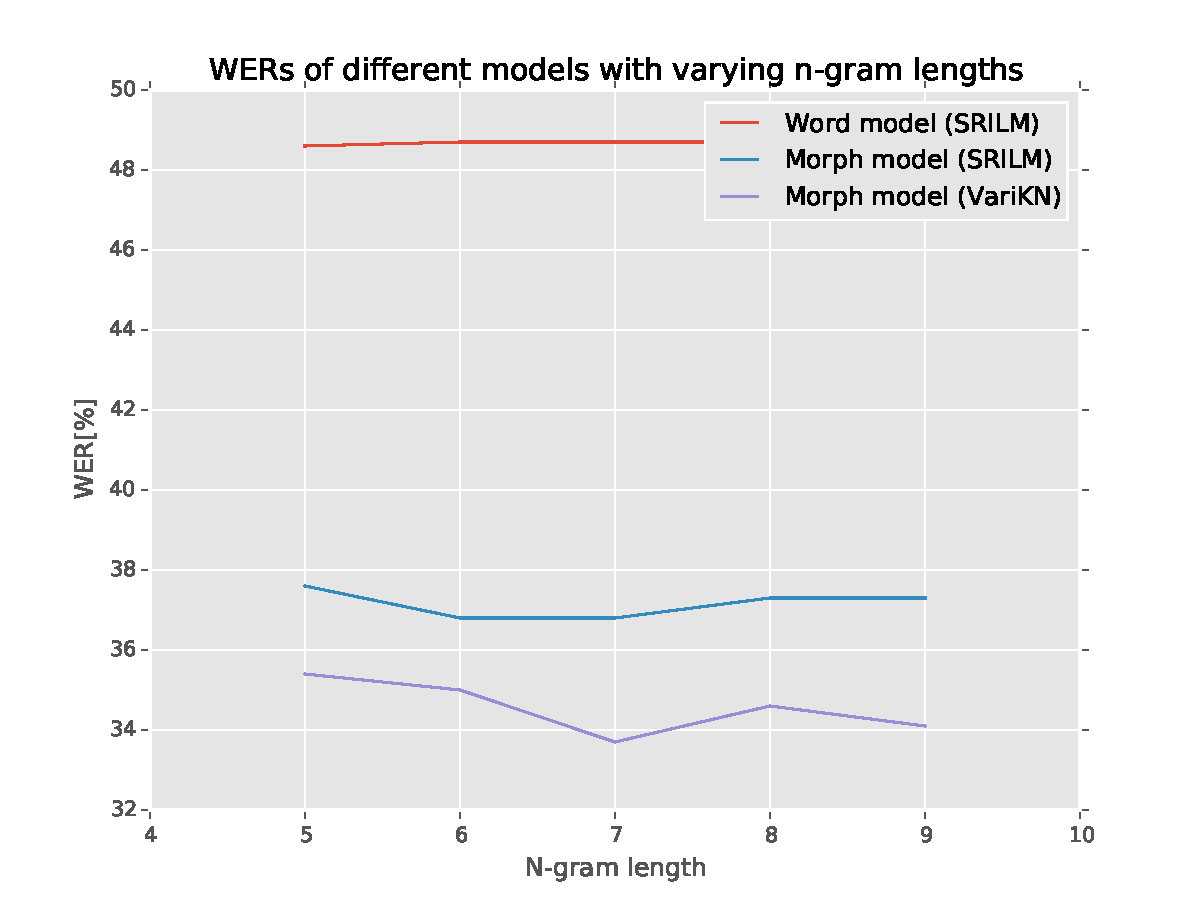
\includegraphics[width=\textwidth]{figures/smeM-complete_wikipedia-wer}
%\caption{Male data - word error rate}
%\end{subfigure}
%
%\end{figure}

\section{Comparsion of low-resource systems for multiple languages}
\label{sec:compexp}
To compare the results of the \ns\ recognizer with recognizers in different languages we first train speaker dependent models for both Finnish and Estonian audiobooks. The available audio datasets are described in Table~\ref{tbl:amdatacomp} and the available text corpora in Table~\ref{tbl:lmdatacomp}.


\begin{table}[!h]
\centering
\begin{tabular}{llllr}
 & \textbf{Language} & \textbf{Gender} & \textbf{Title} & \textbf{Amount}\\\hline
EF1 & Estonian & Female &Nils Holgerssoni imeline teekond läbi Rootsi  & 16 hours \\
EM1 & Estonian & Male & Würst Gabriel ehk Pirita kloostri wiimsed päewad & 6 hours \\
FF1 & Finnish & Female & Syntymättömien sukupolvien Eurooppa & 12 hours\\
FM1 & Finnish & Male & Seitsemän veljestä\footnote{Provided by YLE. Can be listened on  \url{http://areena.yle.fi/1-1301621}} & 13 hours\\
SF1 & \ns & Female & UIT-SME-TTSF & 3.3 hours  \\
SM1 & \ns & Male & UIT-SME-TTSM & 4.6 hours \\
\end{tabular}
\caption{Audio data for the trained speaker dependent systems.\label{tbl:amdatacomp}}
\end{table}

Even though all datasets are audiobooks, there a number of differences. EF1, EM1 and FM1 were encoded in mp3-format, while for the FF1, SM1 and SF1 audiobooks original high quality wav files were available. The speaking style was generally the same, with a story-telling prosody. The exception to this was the FF1 book, an audiobook created for blind persons, which has been read in a very monotone voice with little prosodic variation. This makes the book also understandable when played at higher speeds.

\begin{table}[!h]
\centering
\begin{tabular}{llrrr}
\textbf{Language} & \textbf{Source} & \textbf{\#sentences} & \textbf{ \#word tokens} & \textbf{\#word types}\\\hline
Estonian & Wikipedia &  895k & 10M & 778k \\
 Estonian & newspaper+web+broadcast \cite{kurimo2015modeling} & 19M  & 229M  & 3.8M \\
 Finnish & Wikipedia &  2.2M  & 22M & 1.5M \\
 Finnish & Kielipankki & 13M &  143M & 4.1M \\
 \ns & Wikipedia & 10k & 88k & 20k\\
 \ns & Den samiske tekstbanken & 990k & 12M & 475k\\
%Est_wiki & Estonian & Wikipedia &Nils Holgerssoni imeline teekond läbi Rootsi  & 16 hours \\
%Est_ & Estonian & Male & Würst Gabriel ehk Pirita kloostri wiimsed päewad & 6 hours \\
%FinF & Finnish & Female & Syntymättömien sukupolvien Eurooppa & 12 hours\\
%FinM & Finnish & Male & Seitsemän veljestä & 13 hours\\
%SmeF & \ns & Female & &  \\
%SmeM & \ns & Male & & \\
\end{tabular}
\caption{Language modeling data for the trained speaker dependent systems.\label{tbl:lmdatacomp}}
\end{table}

As the experiments in Section~\ref{sec:samiexp} have confirmed the hypothesis that morph-based n-gram models trained with VariKN give the best performance only this combination will be tested.

To compare the systems fairly, we artifically reduce the amount of audio an text data to mach that of our smallest system. We only use 2.5 hours of audio data and a random 10.000 sentences of the wikipedia data set for each language. The systems are trained with a 10-gram VariKN subword language model. The statistics in Table~\ref{tbl:lmdatacomp_small} show that the datasets are equal in amount of sentences, but not in numbers of word types and tokens. This is most likely because the \ns\ wikipedia has more stub articles that contain short sentences with similar words.

\begin{table}[!h]
\centering
\begin{tabular}{llrrr}
\textbf{Language} & \textbf{\#sentences} & \textbf{\#word tokens} & \textbf{\#word types}\\\hline
Estonian &   10k & 108k & 41k \\
 Finnish &   10k  & 103k & 43k \\
 \ns &  10k & 88k & 20k\\
%Est_wiki & Estonian & Wikipedia &Nils Holgerssoni imeline teekond läbi Rootsi  & 16 hours \\
%Est_ & Estonian & Male & Würst Gabriel ehk Pirita kloostri wiimsed päewad & 6 hours \\
%FinF & Finnish & Female & Syntymättömien sukupolvien Eurooppa & 12 hours\\
%FinM & Finnish & Male & Seitsemän veljestä & 13 hours\\
%SmeF & \ns & Female & &  \\
%SmeM & \ns & Male & & \\
\end{tabular}
\caption{Reduced subsets of wikipedia data for use in the \ds{Train+Wiki} language model.\label{tbl:lmdatacomp_small}}
\end{table}

The results of the comparable systems with the \ds{Train+Wiki} dataset are shown in Table~\ref{tbl:resultssmallcomp}. The word error rates are very close to another, confirming that the systems are comparable. One exception is the FF1 systems, which performs much better. This better result is most likely a combination of very good quality recording and a better match between the text of the language model and the test data.

We also tested the models with the same amount of acoustic data and their respective \ds{Big} language models. The improvements are very significant with the best being 64\% relative improvement in WER for the FF1 system. This shows the importance of the availability of high quality language model data for the performance of a Uralic speech recognition system. The amount of data however is less important, as the \ds{Big} language model for \ns\ gives a similar improvement as the \ds{Big} language models for the other systems, even though the amount of data in the \ds{Big} language model for \ns\ is lower than the amount of data in the \ds{Train+Wiki} systems for Estonian and Finnish.

\begin{table}[!h]
\centering
\begin{tabular}{ll|rr|rr}
 & & \multicolumn{2}{|c|}{\textbf{\ds{Train+Wiki}}}  & \multicolumn{2}{|c}{\textbf{\ds{Big}}}\\
\textbf{Language} & \textbf{Voice} & \textbf{WER} & \textbf{LER}& \textbf{{WER}} & \textbf{LER}\\\hline
Estonian & EF1 & 39.6 & 15.8 & 25.0 & 11.4\\
Estonian & EM1 & 39.2 & 13.3 & 25.5 & 9.6\\
Finnish & FF1 & 25.2 &4.1& 8.9 & 2.1  \\
Finnish & FM1 & 35.8 & 7.7 & 24.9 &  5.6 \\
\ns & SF1 & 37.5 & 8.5 & 23.7  & 5.5 \\
\ns & SM1 & 39.5 & 9.4& 20.9 & 4.9  \\
\end{tabular}
\caption{Word Error Rates for using 2.5 hours of training data and either the \ds{Train+Wiki} or \ds{Big} language models. All language models were 10-gram VariKN subword models, with a 3-gram lookahead model.\label{tbl:resultssmallcomp}}
\end{table}

To see the effect of using more acoustic data, we also trained all systems on their full acoustic datasets and evaluated them with the \ds{Big} language model. Whereas the 2.5 hour data systems were all modeled with appr. 7500 gaussians, the bigger models have proportionally more. 

The results are shown in Table~\ref{tbl:resultbigcomp}.  There are a couple of suprising results. For the FF1 system, there is a little improvement on the already very good result. On the other hand, the SM1 already improves with 13\% relative WER with only an hour of added data. In general there is a clear pattern that more acoustic data will improve the model, but that the effects can be limited if the system has already a good model with just 2.5 hours of data.



%\begin{table}[!h]
%\centering
%\begin{tabular}{llrr}
%\textbf{Language} & \textbf{Gender} & \textbf{Word Error Rate} & \textbf{Letter Error Rate}\\\hline
%Estonian & Female & 39.6 & 15.8 \\
%Estonian & Male & 44.0 & 16.5\\
%Finnish & Female & 25.2 &4.1 \\
%Finnish & Male &  35.8 & 7.7 \\
%\ns & Female & 37.5 & 8.5 \\
%\ns & Male & 39.5 & 9.4 \\
%\end{tabular}
%\caption{Speech recognizer results for the smallest audio dataset with the bigger language model \label{tbl:resultssmallcomp}}
%\end{table}


\begin{table}[!ht]
\centering
\begin{tabular}{llrr|rr|rr}
& & & & \multicolumn{2}{|c}{\textbf{2.5 hours}} & \multicolumn{2}{|c}{\textbf{All data}} \\
\textbf{Language} & \textbf{Voice} & \textbf{\#hours}  &\textbf{\#gaussians} & \textbf{WER} & \textbf{LER}& \textbf{{WER}} & \textbf{LER} \\\hline %& \textbf{\%+ hours} & \textbf{-WER/hour} \\\hline
Estonian & EF1 & 8 &31.5k & 25.0  & 11.4 & 18.8 & 8.3  \\
Estonian & EM1& 4.5& 12.6k&25.5 & 9.6  & 23.2 & 8.4  \\
Finnish & FF1 & 9 & 26k & 8.9 & 2.1  & 8.1 &  1.9  \\
Finnish & FM1 & 10 & 28k & 24.9 & 5.6  & 19.8  & 3.7    \\
\ns & SF1 & 2.5   & 7.7k & 23.7  & 5.5  & 23.7  & 5.5  \\
\ns &SM1 & 3.5 &9.6k & 20.9 & 4.9  & 18.1  & 4.2   \\
\end{tabular}
\caption{Speech recognizer results for the full audio books with the \ds{Big} language model.\label{tbl:resultbigcomp}}
\end{table}

%\note{Compare here the results of all the audio data to the small set. Note how little the FF1 actually gained. EF1 on the other hand benefitted a lot from extra audio data}


\subsection{State of the art recognizers}
The experiments in the previous sections show that results on Finnish and Estonian systems are comparable with \ns\ systems if the same amount of data is provided. This allows us to look to the state-of-the-art recognitions systems for Finnish and Estonian systems and project how well a \ns\ system would perform if the same amount of data would be collected.

\begin{table}[!h]
\centering
\begin{tabular}{llrrl}
\textbf{Language} & \textbf{Description} & \textbf{WER} & \textbf{LER} & \textbf{Source}\\\hline
Estonian & Broadcast conversations  & 17.9\% & &  \cite{alumae2014recent} \\
Estonian & Oral presentations  & 26.3\% & & \cite{alumae2014recent} \\
Finnish & Speecon testset  & & 2.9\%&  \cite{pylkkonen2012} \\
Estonian & Telephone speech &21.6\% & 11.9\% & \cite{hirsimaki2009importance}\\
Finnish & Telephone speech & 33.1\% & 6.8\% & \cite{hirsimaki2009importance}\\
\end{tabular}
\caption{State of the art results for Finnish and Estonian Speaker Independent ASR.}\label{tbl:stateoftheart}
\end{table}

Table~\ref{tbl:stateoftheart} shows the reported error rates for different Speaker Independent systems. The most important difference with the systems discussed in the previous sections is that these are Speaker Independent recognizers, which are tested with different speakers than those present in the training data. Also the quality and type of speech are different.


%\todo{P}{Mention different number of Gaussians or remove reference in Acoustic Modeling section}



\section{Conclusions} 
We have trained Speaker Dependent speech recognitions systems for \ns, and under-resourced Uralic language, and achieved a letter error rate of only 4.2\%. To put this result in perspective and validate the techniques used for training a systems for under-resourced languages we also trained systems for Finnish and Estonian using artificially limited datasets. These experiments have shown that the \ns\ recognizer gives comparable results as Finnish and Estonion recognizers and needs similar techniques such as subword language models.


In future work we plan to use cross-lingual techniques to also build speaker independent systems for \ns, even though the available acoustic datasets might not be available, or available without transcriptions.



%\note{Report the basic results on a Sami SD speech recognizer. Compare them with same condition Finnish and Estonian recognizer. Show the potential for SD systems by extrapolating to full audio book results for Finnish and Estonian and show the potentail to SI system by simply reporting previous results}

%\note{Future work is developing more methods to make an SI recognizer using only limited data, e.g. by using foreign data in AM training}

\section{Acknowledgements} 
We thank Kristiina Jokinen for her help in providing linguistic expertise for \ns. We thank the University of Tromsø for the access to their \ns\ datasets.  This research has been supported by the Academy of Finland under the Finnish Centre of Excellence Program 2012--2017 (grant n\textdegree251170, COIN).
We acknowledge the computational resources provided by the Aalto Science-IT project. 



\bibliographystyle{unsrt}
\bibliography{mybib} 

\end{document}